% \begin{frame}{\tciv{} \dqnes{}}
%     \onslide<2->{
%     \begin{figure}
%     \centering
%     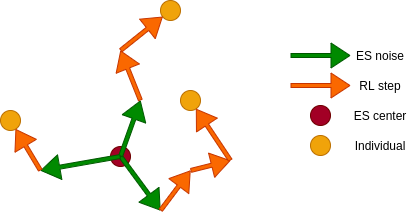
\includegraphics[width=.7\linewidth]{images/DQNES/scheduled.drawio.png}
%     \caption{Distribution of weight values in networks evolved with different encodings.}
%     \end{figure}
%     }
% \end{frame}

\begin{frame}{\tciv{} Using samples to drive the search}%
    \begin{figure}

        \tikzset{every picture/.style={line width=0.75pt}} %set default line width to 0.75pt        

        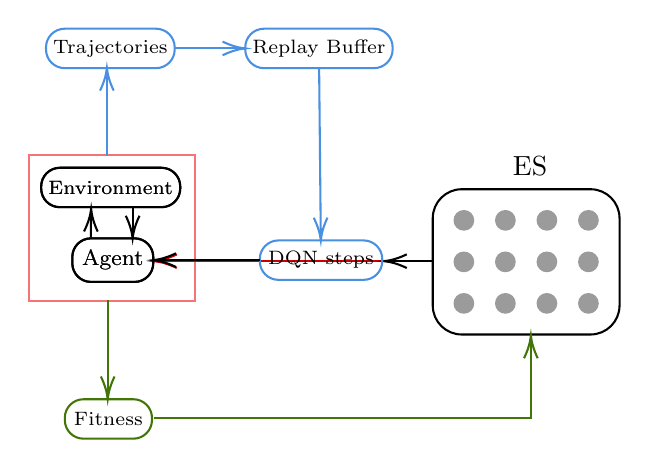
\begin{tikzpicture}[x=0.75pt,y=0.75pt,yscale=-1,xscale=1]
        %uncomment if require: \path (0,300); %set diagram left start at 0, and has height of 300
        \onslide<2->{
            %Rounded Rect [id:dp8415545077066978] 
            \draw   (362.83,123.83) .. controls (362.83,116.1) and (369.1,109.83) .. (376.83,109.83) -- (438.83,109.83) .. controls (446.57,109.83) and (452.83,116.1) .. (452.83,123.83) -- (452.83,165.83) .. controls (452.83,173.57) and (446.57,179.83) .. (438.83,179.83) -- (376.83,179.83) .. controls (369.1,179.83) and (362.83,173.57) .. (362.83,165.83) -- cycle ;
            %Shape: Circle [id:dp8681556448217271] 
            \draw  [draw opacity=0][fill={rgb, 255:red, 155; green, 155; blue, 155 }  ,fill opacity=1 ] (372.83,124.83) .. controls (372.83,122.07) and (375.07,119.83) .. (377.83,119.83) .. controls (380.59,119.83) and (382.83,122.07) .. (382.83,124.83) .. controls (382.83,127.59) and (380.59,129.83) .. (377.83,129.83) .. controls (375.07,129.83) and (372.83,127.59) .. (372.83,124.83) -- cycle ;
            %Shape: Circle [id:dp8988145115218552] 
            \draw  [draw opacity=0][fill={rgb, 255:red, 155; green, 155; blue, 155 }  ,fill opacity=1 ] (372.83,144.83) .. controls (372.83,142.07) and (375.07,139.83) .. (377.83,139.83) .. controls (380.59,139.83) and (382.83,142.07) .. (382.83,144.83) .. controls (382.83,147.59) and (380.59,149.83) .. (377.83,149.83) .. controls (375.07,149.83) and (372.83,147.59) .. (372.83,144.83) -- cycle ;
            %Shape: Circle [id:dp4533836036816683] 
            \draw  [draw opacity=0][fill={rgb, 255:red, 155; green, 155; blue, 155 }  ,fill opacity=1 ] (372.83,164.83) .. controls (372.83,162.07) and (375.07,159.83) .. (377.83,159.83) .. controls (380.59,159.83) and (382.83,162.07) .. (382.83,164.83) .. controls (382.83,167.59) and (380.59,169.83) .. (377.83,169.83) .. controls (375.07,169.83) and (372.83,167.59) .. (372.83,164.83) -- cycle ;
            %Shape: Circle [id:dp16631886989634548] 
            \draw  [draw opacity=0][fill={rgb, 255:red, 155; green, 155; blue, 155 }  ,fill opacity=1 ] (392.83,124.83) .. controls (392.83,122.07) and (395.07,119.83) .. (397.83,119.83) .. controls (400.59,119.83) and (402.83,122.07) .. (402.83,124.83) .. controls (402.83,127.59) and (400.59,129.83) .. (397.83,129.83) .. controls (395.07,129.83) and (392.83,127.59) .. (392.83,124.83) -- cycle ;
            %Shape: Circle [id:dp5655160494827564] 
            \draw  [draw opacity=0][fill={rgb, 255:red, 155; green, 155; blue, 155 }  ,fill opacity=1 ] (392.83,144.83) .. controls (392.83,142.07) and (395.07,139.83) .. (397.83,139.83) .. controls (400.59,139.83) and (402.83,142.07) .. (402.83,144.83) .. controls (402.83,147.59) and (400.59,149.83) .. (397.83,149.83) .. controls (395.07,149.83) and (392.83,147.59) .. (392.83,144.83) -- cycle ;
            %Shape: Circle [id:dp7156251851857748] 
            \draw  [draw opacity=0][fill={rgb, 255:red, 155; green, 155; blue, 155 }  ,fill opacity=1 ] (392.83,164.83) .. controls (392.83,162.07) and (395.07,159.83) .. (397.83,159.83) .. controls (400.59,159.83) and (402.83,162.07) .. (402.83,164.83) .. controls (402.83,167.59) and (400.59,169.83) .. (397.83,169.83) .. controls (395.07,169.83) and (392.83,167.59) .. (392.83,164.83) -- cycle ;
            %Shape: Circle [id:dp7494124641564217] 
            \draw  [draw opacity=0][fill={rgb, 255:red, 155; green, 155; blue, 155 }  ,fill opacity=1 ] (412.83,124.83) .. controls (412.83,122.07) and (415.07,119.83) .. (417.83,119.83) .. controls (420.59,119.83) and (422.83,122.07) .. (422.83,124.83) .. controls (422.83,127.59) and (420.59,129.83) .. (417.83,129.83) .. controls (415.07,129.83) and (412.83,127.59) .. (412.83,124.83) -- cycle ;
            %Shape: Circle [id:dp3773090392829881] 
            \draw  [draw opacity=0][fill={rgb, 255:red, 155; green, 155; blue, 155 }  ,fill opacity=1 ] (412.83,144.83) .. controls (412.83,142.07) and (415.07,139.83) .. (417.83,139.83) .. controls (420.59,139.83) and (422.83,142.07) .. (422.83,144.83) .. controls (422.83,147.59) and (420.59,149.83) .. (417.83,149.83) .. controls (415.07,149.83) and (412.83,147.59) .. (412.83,144.83) -- cycle ;
            %Shape: Circle [id:dp9928212769981617] 
            \draw  [draw opacity=0][fill={rgb, 255:red, 155; green, 155; blue, 155 }  ,fill opacity=1 ] (412.83,164.83) .. controls (412.83,162.07) and (415.07,159.83) .. (417.83,159.83) .. controls (420.59,159.83) and (422.83,162.07) .. (422.83,164.83) .. controls (422.83,167.59) and (420.59,169.83) .. (417.83,169.83) .. controls (415.07,169.83) and (412.83,167.59) .. (412.83,164.83) -- cycle ;
            %Shape: Circle [id:dp9943772010153576] 
            \draw  [draw opacity=0][fill={rgb, 255:red, 155; green, 155; blue, 155 }  ,fill opacity=1 ] (432.83,124.83) .. controls (432.83,122.07) and (435.07,119.83) .. (437.83,119.83) .. controls (440.59,119.83) and (442.83,122.07) .. (442.83,124.83) .. controls (442.83,127.59) and (440.59,129.83) .. (437.83,129.83) .. controls (435.07,129.83) and (432.83,127.59) .. (432.83,124.83) -- cycle ;
            %Shape: Circle [id:dp5095085253879101] 
            \draw  [draw opacity=0][fill={rgb, 255:red, 155; green, 155; blue, 155 }  ,fill opacity=1 ] (432.83,144.83) .. controls (432.83,142.07) and (435.07,139.83) .. (437.83,139.83) .. controls (440.59,139.83) and (442.83,142.07) .. (442.83,144.83) .. controls (442.83,147.59) and (440.59,149.83) .. (437.83,149.83) .. controls (435.07,149.83) and (432.83,147.59) .. (432.83,144.83) -- cycle ;
            %Shape: Circle [id:dp9842362857007814] 
            \draw  [draw opacity=0][fill={rgb, 255:red, 155; green, 155; blue, 155 }  ,fill opacity=1 ] (432.83,164.83) .. controls (432.83,162.07) and (435.07,159.83) .. (437.83,159.83) .. controls (440.59,159.83) and (442.83,162.07) .. (442.83,164.83) .. controls (442.83,167.59) and (440.59,169.83) .. (437.83,169.83) .. controls (435.07,169.83) and (432.83,167.59) .. (432.83,164.83) -- cycle ;
            % Text Node
            \draw (409.72,98.78) node   [align=left] {ES};
        }
        \onslide<3->{
            % Text Node
            \draw    (189.17,142.5) .. controls (189.17,137.53) and (193.2,133.5) .. (198.17,133.5) -- (219.17,133.5) .. controls (224.14,133.5) and (228.17,137.53) .. (228.17,142.5) -- (228.17,145.5) .. controls (228.17,150.47) and (224.14,154.5) .. (219.17,154.5) -- (198.17,154.5) .. controls (193.2,154.5) and (189.17,150.47) .. (189.17,145.5) -- cycle  ;
            \draw (208.67,144) node  [font=\footnotesize] [align=left] {Agent};
            % Text Node
            \draw    (174.17,108.5) .. controls (174.17,103.53) and (178.2,99.5) .. (183.17,99.5) -- (232.17,99.5) .. controls (237.14,99.5) and (241.17,103.53) .. (241.17,108.5) -- (241.17,109.5) .. controls (241.17,114.47) and (237.14,118.5) .. (232.17,118.5) -- (183.17,118.5) .. controls (178.2,118.5) and (174.17,114.47) .. (174.17,109.5) -- cycle  ;
            \draw (207.67,109) node  [font=\scriptsize] [align=left] {Environment};
            %Shape: Rectangle [id:dp8077403849937568] 
            \draw  [color={rgb, 255:red, 244; green, 116; blue, 116 }  ,draw opacity=1 ] (168.17,93.5) -- (248.17,93.5) -- (248.17,163.5) -- (168.17,163.5) -- cycle ;
            %Straight Lines [id:da03625790155481623] 
            \draw    (218.24,118.35) -- (218.24,131.58) ;
            \draw [shift={(218.24,133.58)}, rotate = 270] [color={rgb, 255:red, 0; green, 0; blue, 0 }  ][line width=0.75]    (10.93,-3.29) .. controls (6.95,-1.4) and (3.31,-0.3) .. (0,0) .. controls (3.31,0.3) and (6.95,1.4) .. (10.93,3.29)   ;
            %Straight Lines [id:da661675132731175] 
            \draw    (198.09,133.12) -- (198.22,121.27) ;
            \draw [shift={(198.24,119.27)}, rotate = 90.64] [color={rgb, 255:red, 0; green, 0; blue, 0 }  ][line width=0.75]    (10.93,-3.29) .. controls (6.95,-1.4) and (3.31,-0.3) .. (0,0) .. controls (3.31,0.3) and (6.95,1.4) .. (10.93,3.29)   ;
        % }
        \onslide<3-4>{
            %Straight Lines [id:da5700505568511188] 
            \draw [color={rgb, 255:red, 205; green, 0; blue, 0 }  ,draw opacity=1 ]   (362.72,144.5) -- (230.6,144.5) ;
            \draw [shift={(228.6,144.5)}, rotate = 360] [color={rgb, 255:red, 205; green, 0; blue, 0 }  ,draw opacity=1 ][line width=0.75]    (10.93,-3.29) .. controls (6.95,-1.4) and (3.31,-0.3) .. (0,0) .. controls (3.31,0.3) and (6.95,1.4) .. (10.93,3.29)   ;}

            % Text Node
            \draw    (189.17,142.5) .. controls (189.17,137.53) and (193.2,133.5) .. (198.17,133.5) -- (219.17,133.5) .. controls (224.14,133.5) and (228.17,137.53) .. (228.17,142.5) -- (228.17,145.5) .. controls (228.17,150.47) and (224.14,154.5) .. (219.17,154.5) -- (198.17,154.5) .. controls (193.2,154.5) and (189.17,150.47) .. (189.17,145.5) -- cycle  ;
            \draw (208.67,144) node  [font=\footnotesize] [align=left] {Agent};
            % Text Node
            \draw    (174.17,108.5) .. controls (174.17,103.53) and (178.2,99.5) .. (183.17,99.5) -- (232.17,99.5) .. controls (237.14,99.5) and (241.17,103.53) .. (241.17,108.5) -- (241.17,109.5) .. controls (241.17,114.47) and (237.14,118.5) .. (232.17,118.5) -- (183.17,118.5) .. controls (178.2,118.5) and (174.17,114.47) .. (174.17,109.5) -- cycle  ;
            \draw (207.67,109) node  [font=\scriptsize] [align=left] {Environment};
            %Straight Lines [id:da29906615776037226] 
            \draw [color={rgb, 255:red, 65; green, 117; blue, 5 }  ,draw opacity=1 ]   (206.23,163.4) -- (206.23,209) ;
            \draw [shift={(206.23,211)}, rotate = 270] [color={rgb, 255:red, 65; green, 117; blue, 5 }  ,draw opacity=1 ][line width=0.75]    (10.93,-3.29) .. controls (6.95,-1.4) and (3.31,-0.3) .. (0,0) .. controls (3.31,0.3) and (6.95,1.4) .. (10.93,3.29)   ;
            %Straight Lines [id:da624160799597017] 
            \draw [color={rgb, 255:red, 65; green, 117; blue, 5 }  ,draw opacity=1 ]   (228.33,220.17) -- (410.11,220.17) -- (410.11,182.33) ;
            \draw [shift={(410.11,180.33)}, rotate = 90] [color={rgb, 255:red, 65; green, 117; blue, 5 }  ,draw opacity=1 ][line width=0.75]    (10.93,-3.29) .. controls (6.95,-1.4) and (3.31,-0.3) .. (0,0) .. controls (3.31,0.3) and (6.95,1.4) .. (10.93,3.29)   ;
            % Text Node
            \draw  [color={rgb, 255:red, 65; green, 117; blue, 5 }  ,draw opacity=1 ]  (185.56,220.02) .. controls (185.56,215.05) and (189.58,211.02) .. (194.56,211.02) -- (218.56,211.02) .. controls (223.53,211.02) and (227.56,215.05) .. (227.56,220.02) -- (227.56,221.02) .. controls (227.56,225.99) and (223.53,230.02) .. (218.56,230.02) -- (194.56,230.02) .. controls (189.58,230.02) and (185.56,225.99) .. (185.56,221.02) -- cycle  ;
            \draw (206.56,220.52) node  [font=\scriptsize] [align=left] {Fitness};
        }
        \onslide<4->{
            %Straight Lines [id:da6625734832851018] 
            \draw [color={rgb, 255:red, 74; green, 144; blue, 226 }  ,draw opacity=1 ]   (205.83,93.67) -- (205.83,53.4) ;
            \draw [shift={(205.83,51.4)}, rotate = 90] [color={rgb, 255:red, 74; green, 144; blue, 226 }  ,draw opacity=1 ][line width=0.75]    (10.93,-3.29) .. controls (6.95,-1.4) and (3.31,-0.3) .. (0,0) .. controls (3.31,0.3) and (6.95,1.4) .. (10.93,3.29)   ;
            % Text Node
            \draw  [color={rgb, 255:red, 74; green, 144; blue, 226 }  ,draw opacity=1 ]  (176.5,41.5) .. controls (176.5,36.53) and (180.53,32.5) .. (185.5,32.5) -- (229.5,32.5) .. controls (234.47,32.5) and (238.5,36.53) .. (238.5,41.5) -- (238.5,42.5) .. controls (238.5,47.47) and (234.47,51.5) .. (229.5,51.5) -- (185.5,51.5) .. controls (180.53,51.5) and (176.5,47.47) .. (176.5,42.5) -- cycle  ;
            \draw (207.5,42) node  [font=\scriptsize] [align=left] {Trajectories};
        }

        \onslide<5->{
            %Straight Lines [id:da9070693346947258] 
            \draw    (362.72,144.5) -- (341.39,144.5) ;
            \draw [shift={(339.39,144.5)}, rotate = 360] [color={rgb, 255:red, 0; green, 0; blue, 0 }  ][line width=0.75]    (10.93,-3.29) .. controls (6.95,-1.4) and (3.31,-0.3) .. (0,0) .. controls (3.31,0.3) and (6.95,1.4) .. (10.93,3.29)   ; 
            % Text Node
            \draw  [color={rgb, 255:red, 74; green, 144; blue, 226 }  ,draw opacity=1 ]  (272.5,41.5) .. controls (272.5,36.53) and (276.53,32.5) .. (281.5,32.5) -- (334.5,32.5) .. controls (339.47,32.5) and (343.5,36.53) .. (343.5,41.5) -- (343.5,42.5) .. controls (343.5,47.47) and (339.47,51.5) .. (334.5,51.5) -- (281.5,51.5) .. controls (276.53,51.5) and (272.5,47.47) .. (272.5,42.5) -- cycle  ;
            \draw (308,42) node  [font=\scriptsize] [align=left] {Replay Buffer};
            % Text Node
            \draw  [color={rgb, 255:red, 74; green, 144; blue, 226 }  ,draw opacity=1 ]  (279.5,143.5) .. controls (279.5,138.53) and (283.53,134.5) .. (288.5,134.5) -- (329.5,134.5) .. controls (334.47,134.5) and (338.5,138.53) .. (338.5,143.5) -- (338.5,144.5) .. controls (338.5,149.47) and (334.47,153.5) .. (329.5,153.5) -- (288.5,153.5) .. controls (283.53,153.5) and (279.5,149.47) .. (279.5,144.5) -- cycle  ;
            \draw (309,144) node  [font=\scriptsize] [align=left] {DQN steps};
            % Connection
            \draw [color={rgb, 255:red, 74; green, 144; blue, 226 }  ,draw opacity=1 ]   (238.5,42) -- (270.5,42) ;
            \draw [shift={(272.5,42)}, rotate = 180] [color={rgb, 255:red, 74; green, 144; blue, 226 }  ,draw opacity=1 ][line width=0.75]    (10.93,-3.29) .. controls (6.95,-1.4) and (3.31,-0.3) .. (0,0) .. controls (3.31,0.3) and (6.95,1.4) .. (10.93,3.29)   ;
            % Connection
            \draw [color={rgb, 255:red, 74; green, 144; blue, 226 }  ,draw opacity=1 ]   (308.09,51.5) -- (308.89,132.5) ;
            \draw [shift={(308.91,134.5)}, rotate = 269.44] [color={rgb, 255:red, 74; green, 144; blue, 226 }  ,draw opacity=1 ][line width=0.75]    (10.93,-3.29) .. controls (6.95,-1.4) and (3.31,-0.3) .. (0,0) .. controls (3.31,0.3) and (6.95,1.4) .. (10.93,3.29)   ;
            % Connection
            \draw    (279.5,144) -- (230.17,144) ;
            \draw [shift={(228.17,144)}, rotate = 360] [color={rgb, 255:red, 0; green, 0; blue, 0 }  ][line width=0.75]    (10.93,-3.29) .. controls (6.95,-1.4) and (3.31,-0.3) .. (0,0) .. controls (3.31,0.3) and (6.95,1.4) .. (10.93,3.29)   ;
        }
            
        \end{tikzpicture}


    \end{figure}
\end{frame}


\begin{frame}{\tciv{} DQNES}%
    \begin{figure}
        
    \tikzset{every picture/.style={line width=0.75pt}} %set default line width to 0.75pt        

    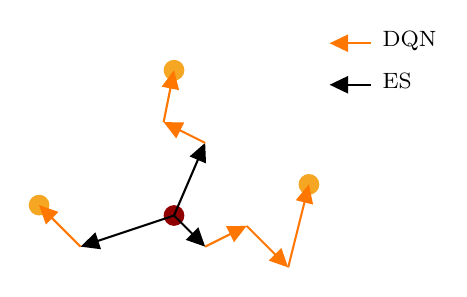
\begin{tikzpicture}[x=0.75pt,y=0.75pt,yscale=-1,xscale=1]
    %uncomment if require: \path (0,300); %set diagram left start at 0, and has height of 300
        % Center
        \onslide<2->{
        %Flowchart: Connector [id:dp7892172092869572] 
        \draw  [draw opacity=0][fill={rgb, 255:red, 145; green, 0; blue, 0 }  ,fill opacity=1 ] (270,155) .. controls (270,152.24) and (272.24,150) .. (275,150) .. controls (277.76,150) and (280,152.24) .. (280,155) .. controls (280,157.76) and (277.76,160) .. (275,160) .. controls (272.24,160) and (270,157.76) .. (270,155) -- cycle ;
        }

        % End points
        \onslide<4->{
        %Flowchart: Connector [id:dp8059049646076628] 
        \draw  [draw opacity=0][fill={rgb, 255:red, 245; green, 166; blue, 35 }  ,fill opacity=1 ] (205,150) .. controls (205,147.24) and (207.24,145) .. (210,145) .. controls (212.76,145) and (215,147.24) .. (215,150) .. controls (215,152.76) and (212.76,155) .. (210,155) .. controls (207.24,155) and (205,152.76) .. (205,150) -- cycle ;
        %Flowchart: Connector [id:dp5011381675096028] 
        \draw  [draw opacity=0][fill={rgb, 255:red, 245; green, 166; blue, 35 }  ,fill opacity=1 ] (270,85) .. controls (270,82.24) and (272.24,80) .. (275,80) .. controls (277.76,80) and (280,82.24) .. (280,85) .. controls (280,87.76) and (277.76,90) .. (275,90) .. controls (272.24,90) and (270,87.76) .. (270,85) -- cycle ;
        %Flowchart: Connector [id:dp3773909027910184] 
        \draw  [draw opacity=0][fill={rgb, 255:red, 245; green, 166; blue, 35 }  ,fill opacity=1 ] (335,140) .. controls (335,137.24) and (337.24,135) .. (340,135) .. controls (342.76,135) and (345,137.24) .. (345,140) .. controls (345,142.76) and (342.76,145) .. (340,145) .. controls (337.24,145) and (335,142.76) .. (335,140) -- cycle ;
        }

        \onslide<3->{
        %Straight Lines [id:da6809885341795275] 
        \draw    (275,155) -- (232.85,169.05) ;
        \draw [shift={(230,170)}, rotate = 341.57] [fill={rgb, 255:red, 0; green, 0; blue, 0 }  ][line width=0.08]  [draw opacity=0] (8.93,-4.29) -- (0,0) -- (8.93,4.29) -- cycle    ;
        %Straight Lines [id:da34929359178134534] 
        \draw    (275,155) -- (288.82,122.76) ;
        \draw [shift={(290,120)}, rotate = 113.2] [fill={rgb, 255:red, 0; green, 0; blue, 0 }  ][line width=0.08]  [draw opacity=0] (8.93,-4.29) -- (0,0) -- (8.93,4.29) -- cycle    ;
        %Straight Lines [id:da4067586836296815] 
        \draw    (275,155) -- (287.88,167.88) ;
        \draw [shift={(290,170)}, rotate = 225] [fill={rgb, 255:red, 0; green, 0; blue, 0 }  ][line width=0.08]  [draw opacity=0] (8.93,-4.29) -- (0,0) -- (8.93,4.29) -- cycle    ;
        %Straight Lines [id:da7752837053635281] 
        \draw    (370,92) -- (353,92) ;
        \draw [shift={(350,92)}, rotate = 360] [fill={rgb, 255:red, 0; green, 0; blue, 0 }  ][line width=0.08]  [draw opacity=0] (8.93,-4.29) -- (0,0) -- (8.93,4.29) -- cycle    ;
        % Text Node
        \draw (374,85) node [anchor=north west][inner sep=0.75pt]  [font=\footnotesize] [align=left] {ES};
        }

        \onslide<4->{
        %Straight Lines [id:da5651183383226251] 
        \draw [color={rgb, 255:red, 255; green, 118; blue, 0 }  ,draw opacity=1 ]   (230,170) -- (212.12,152.12) ;
        \draw [shift={(210,150)}, rotate = 45] [fill={rgb, 255:red, 255; green, 118; blue, 0 }  ,fill opacity=1 ][line width=0.08]  [draw opacity=0] (8.93,-4.29) -- (0,0) -- (8.93,4.29) -- cycle    ;
        %Straight Lines [id:da9174794629852384] 
        \draw [color={rgb, 255:red, 255; green, 118; blue, 0 }  ,draw opacity=1 ]   (290,170) -- (307.32,161.34) ;
        \draw [shift={(310,160)}, rotate = 153.43] [fill={rgb, 255:red, 255; green, 118; blue, 0 }  ,fill opacity=1 ][line width=0.08]  [draw opacity=0] (8.93,-4.29) -- (0,0) -- (8.93,4.29) -- cycle    ;
        %Straight Lines [id:da9236788570029154] 
        \draw [color={rgb, 255:red, 255; green, 118; blue, 0 }  ,draw opacity=1 ]   (310,160) -- (327.88,177.88) ;
        \draw [shift={(330,180)}, rotate = 225] [fill={rgb, 255:red, 255; green, 118; blue, 0 }  ,fill opacity=1 ][line width=0.08]  [draw opacity=0] (8.93,-4.29) -- (0,0) -- (8.93,4.29) -- cycle    ;
        %Straight Lines [id:da5363883614541579] 
        \draw [color={rgb, 255:red, 255; green, 118; blue, 0 }  ,draw opacity=1 ]   (330,180) -- (339.27,142.91) ;
        \draw [shift={(340,140)}, rotate = 104.04] [fill={rgb, 255:red, 255; green, 118; blue, 0 }  ,fill opacity=1 ][line width=0.08]  [draw opacity=0] (8.93,-4.29) -- (0,0) -- (8.93,4.29) -- cycle    ;
        %Straight Lines [id:da8537813572490652] 
        \draw [color={rgb, 255:red, 255; green, 118; blue, 0 }  ,draw opacity=1 ]   (290,120) -- (272.68,111.34) ;
        \draw [shift={(270,110)}, rotate = 26.57] [fill={rgb, 255:red, 255; green, 118; blue, 0 }  ,fill opacity=1 ][line width=0.08]  [draw opacity=0] (8.93,-4.29) -- (0,0) -- (8.93,4.29) -- cycle    ;
        %Straight Lines [id:da4405746369803901] 
        \draw [color={rgb, 255:red, 255; green, 118; blue, 0 }  ,draw opacity=1 ]   (270,110) -- (274.41,87.94) ;
        \draw [shift={(275,85)}, rotate = 101.31] [fill={rgb, 255:red, 255; green, 118; blue, 0 }  ,fill opacity=1 ][line width=0.08]  [draw opacity=0] (8.93,-4.29) -- (0,0) -- (8.93,4.29) -- cycle    ;
        %Straight Lines [id:da8366023954327625] 
        \draw [color={rgb, 255:red, 255; green, 118; blue, 0 }  ,draw opacity=1 ]   (370,72) -- (353,72) ;
        \draw [shift={(350,72)}, rotate = 360] [fill={rgb, 255:red, 255; green, 118; blue, 0 }  ,fill opacity=1 ][line width=0.08]  [draw opacity=0] (8.93,-4.29) -- (0,0) -- (8.93,4.29) -- cycle    ;
        
        % Text Node
        \draw (374,65) node [anchor=north west][inner sep=0.75pt]  [font=\footnotesize] [align=left] {DQN};
        }

\end{tikzpicture}

    \end{figure}
\end{frame}

